%%================================================
%% Filename: chap02.tex
%% Encoding: UTF-8
%% Author: Yuan Xiaoshuai - yxshuai@gmail.com
%% Created: 2012-04-27 19:37
%% Last modified: 2019-11-05 23:57
%%================================================
\chapter{相关理论知识与关键技术}
\label{cha:basic-knowledge}
  
\section{源地址伪造攻击的分类}

源地址伪造攻击可以根据伪造产生的虚假地址与攻击者受害者所在网络的关系来进行分类,总共可分为六类:
a.虚假地址在网络中不存在或已经失活;
b.虚假地址指向的主机是受害者;
c.虚假地址与受害者主机处于同一个子网中;
d.虚假地址与攻击者处于同一个子网中;
e.虚假地址处于攻击者和受害者之间的路径中;
f.虚假地址既不在攻击者与受害者的子网中也不在攻击者与受害者之间的路径当中\onlinecite{Bi2010}。
以下是这六类攻击的详细描述,表~\ref{tab:source_address_spoofing}~展示了这六种攻击之间的关系。

\subsection*{a类}
 恶意主机通过产生随机的互联网中不存在的或着已经失效的IP地址来对攻击数据包的源地址进行伪造。
 产生的攻击数据包占用着受害者主机的资源,使受害者不能再向其他主机提供服务。
 这些IP地址包括RFC1918中指定的私有IP地址\cite{Rekhter1996}、RFC3330中的自动分配的IP地址\cite{BogonList2003}、循环测试地址,这些IP地址都不会在互联网中出现。
SYN Flood是一种常见的攻击方式,它能够不断消耗受害者主机CPU资源以及内存资源并阻止其他合法用户的连接。
在不设置保护策略的情况下,少量的SYN洪水攻击便足以使受害者主机崩溃。
由于受害者主机在受到攻击时会向恶意数据包中源地址指向的主机返回SYNACK包使其返回RTS包释放半连接。
这就导致了此种攻击的虚假地址将会采用上面所说的地址。
\subsection*{b类}
攻击者将受害者主机的IP地址作为攻击数据包的源地址以此来实现反射性攻击、直接攻击和诱捕攻击,这类攻击通常有三种形式:
攻击数据包的源地址是受害者主机IP地址,目标地址是受害者主机的所在子网的广播地址。
攻击数据包被广播之后,受害者将收到大量的ACK回复,这会使受害者淹没于这些流量当中而大大地削弱了受害者的正常服务能力。
攻击数据包的源地址与目标地址同时是受害者主机的IP,受害者收到攻击数据包后会将其响应发送给自己,这一行为会导致受害者受到干扰而瘫痪。
著名的DrDoS\cite{Gibson2002}是此类攻击的一个典型例子,它会使受害者的带宽或内存等资源溢出或者过载而不能使用。
TFN\cite{Dittrich1999}和Land  attacks\cite{CERT1997}也是此类典型的例子。
攻击者向受害者发送数据包,其源主机/端口与目标主机/端口相同,并设置了SYN标志能够锁死受害者或使其协议栈崩溃。
\subsection*{c类}
此类攻击将受害者所处子网中的IP地址作为攻击数据包中的源地址,并依赖于受害者和虚假地址所指向的主机之间的信任关系。
基于TCP连接的盲IP欺骗攻击\cite{Ali2007}是这类攻击的典型例子。
TFN2K\cite{Barlow2000}也是一个例子,它是TFN\cite{Dittrich1999}的下一代版本。
\subsection*{d类}
d类攻击将攻击者所处子网内的地址作为源地址,因为入口过滤的粒度通常不高便可以很容易使攻击数据包通过入口过滤。
反弹扫描\cite{CERT1997}是这类产品的一个典型例子,为了从受害者那里获取响应包,攻击者伪造同一子网络中邻居的源地址,并嗅探返回给邻居的流量数据。
这种攻击可用于端口扫描,如果受害者的一个端口被关闭,受害者将回复RST数据包\cite{Ray1981},更糟糕的是,这种攻击可以有效地逃脱uRPF的攻击\cite{CiscoIOS2005}。
\subsection*{e类}
攻击者通常强迫网络设备的源地址出现在攻击者与受害者之间的路径上。
在这种类型的攻击下,攻击者可以传播虚假的DNS或路由信息,并重定向网络流量\onlinecite{Huang2006}。这将被认为是最危险的袭击之一。
\subsection*{f类}
攻击者不依赖于受害者和虚假地址之间的特殊拓扑关系。
这类攻击通常被组合在一起,例如MITM攻击\cite{ManInTheMiddle2007}是两种典型的f类攻击的一种组合。
如A分别与V1和V2进行通信,则A在与V2通信时伪造V1的源地址,在与V1通信时伪造V2的源地址。

\begin{table}[htbp]
    \caption{源地址伪造攻击分类}
    \label{tab:source_address_spoofing}
    \centering
    \begin{tabular}{cccc}
    \toprule
    {\heiti 分类} & {\heiti 虚假地址状态} & {\heiti 与攻击者关系} & {\heiti 与受害者关系}  \\ 
    \midrule
    a类 & 不存在或已经失活 & 无 & 无 \\ 
    b类 & 存在 & 无 & 指向 \\ 
    c类 & 存在 & 无 & 同子网 \\ 
    d类 & 存在 & 同子网 & 无 \\ 
    e类 & 存在 & 攻击者到受害路径内 & 攻击者到受害者路径内 \\ 
    f类 & 不存在 & 无 & 无 \\ 
    \bottomrule
    \end{tabular}
    \end{table}

\section{数据包标记法}
图~\ref{fig:simple_topology}~是一个IP回溯问题的简单网络拓扑图。
\begin{figure}[htbp]
  \centering
  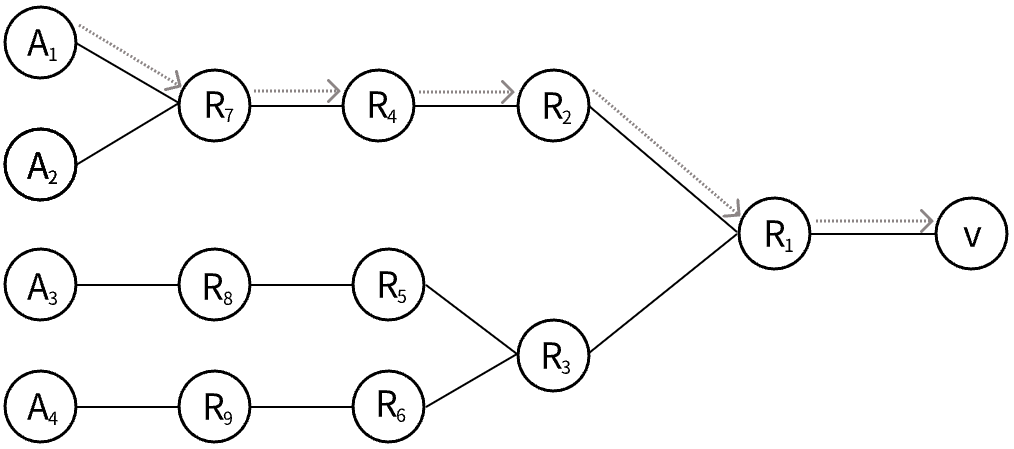
\includegraphics[width = 0.8\textwidth]{simple_topology.png}
  \caption{针对路由回溯问题的简单拓扑图}
  \label{fig:simple_topology}
\end{figure}
整个结构可以看作是一棵以$V$为根节点的树,$V$代表一个遭受攻击的\textbf{受害者},它可能为服务器、防火墙或者入侵检测系统。
每个$A_i$是树中的叶子节点,它代表潜在的\textbf{攻击源},它可能为例如攻击者主机也可能为普通的用户。
每个$R_i$则代表从这些$A_i$到$V$的中间路由器。
在这个网络中,每个$A_i$都有可能向$V$发送数据包,而这些数据包中则有潜在攻击数据包的可能性。
其中这些攻击数据包走过的路径都为\textbf{攻击路径},它是一个从攻击节点$A_i$到$V$的有序唯一路由序列。
例如,假设$A_1$是一个攻击节点,它正在向$V$发送攻击数据包,这些攻击数据包走过的路径是唯一的,由$R_7$、$R_4$、$R_2$、$R_1$依次组成,则这条从$A_1$到$V$的唯一的路径就是一条攻击路径。
一个\textbf{IP回溯问题}就是通过一些方法和策略确定攻击路径,揭示攻击主机的真实身份和具体位置。



当回溯成功后便可以从攻击源的下游最近邻路由器过滤掉这些数据包以保护受害者服务器免受攻击。
在这个问题中,似乎只要从攻击数据包中提取出源IP就可以确定攻击路径,然而解决这个问题通常是很复杂的。
一个有预谋、有准备的攻击通常会做出一些手段,例如伪造攻击数据包的源IP地址、发送一些虚假信息来伪造攻击路径从而干扰溯源,使溯源任务极难完成。



一个IP回溯问题相对简单的近似溯源为找到一条包含有真实攻击路径作为路径后缀的候选路径,这个路径后缀就是有效后缀\cite{savage2000practical}。
例如,$R_8$、$R_5$、$R_3$、$R_7$、$R_4$、$R_2$、$R_1$就是一条有效的候选路径,因为它包含$R_7$、$R_4$、$R_2$、$R_1$这条真实的攻击路径作为候选路径的后缀。
而在接下来的本方案描述中却可以确定真实的攻击路径而不仅仅是候选路径,这是本方案的一大优势,这往往往需要网络中间设备来协作配合。



数据包标记法通常由两部分组成,即\textbf{标记过程}和\textbf{路径重组过程}。
当部署了本方案的路由器$R_i$接收到数据包后,便会执行标记过程。
在标记过程中,路由器$R_i$通过向待转发的数据包注入额外的标记信息来记录自身路由信息。
这些标记信息类型可能为路由器IP地址也可能是其他一些控制信息类型,具体的标记信息类型根据所选的方案而异。
通常,这些信息被注入到数据包的头部字段中,图~\ref{fig:ipv4_header}~显示了数据包头部字段被用作标记字段的情况。
当受害者$V$成功收集到足够数量的标记数据包以满足回溯需求时,系统将进入\textbf{收敛状态}。



在收敛状态下,受害者所收集的标记数据包数量已完全能够支撑受害者主机完成路由回溯。
在传统的概率包标记法中,路由器$R_i$距离受害者$V$越远,受害者$V$收集到$R_i$所标记的数据包概率将越小。
因此,受害者$V$收集的数据包为距自身最远路由器$R_i$所标记的概率是最小的,为$p(1-p)^(d-1)$。
通常情况下,要达到收敛状态所需的最少数据包数量将由此概率决定,为$\frac{1}{p(1-p)^(d-1)}$。
受害者$V$一旦达到收敛状态后,便可根据这些标记信息使用一定的算法来执行路径重构过程,即受害者$V$会根据受到的标记信息执行相应算法找到攻击源。

\section{遗传算法\cite{zhou2006matlab}}
\label{sec:GA}
\subsection{遗传算法概述}
遗传算法(Genetic Algorithm,简称GA)是一种搜索启发式算法,受到生物进化理论的启发。
它通过模拟模拟自然界中生物进化的机制,如\textbf{遗传(Heredity)}、\textbf{变异(Mutation)}、\textbf{交配(Crossover )}和\textbf{选择(Selection)}来解决优化和搜索问题。


算法从一个随机生成的\textbf{初始种群(Population)}开始,种群中的每个个体代表了问题空间中的一个潜在解决方案,并以某种方式(通常是数值或结构形式)编码。
每个个体的\textbf{适应度}被评估,以确定其在给定问题中的效用。
遗传算法然后使用遗传操作符选择\textbf{最适合的个体(Individual)}进行交叉和变异,以产生新一代种群。
这个过程重复进行,直到满足终止条件(如达到一定的迭代次数或解的质量)。


遗传算法被广泛应用于各种领域,包括优化问题、机器学习、调度和人工智能,因为它们对初解的质量不敏感,且能在复杂的、多峰值的搜索空间中找到全局最优解。
由于遗传算法是由进化论和遗传学机理而产生的搜索算法,所以在这个算法中会用到一些生物遗传学知识,下面是遗传算法中的一些常用术语。
\begin{enumerate}
  \item \textbf{种群(Population):}一个种群由多个个体组成,每个个体代表了问题空间中的一个可能解。

  \item \textbf{个体(Individual):}在遗传算法中,个体通常用一个字符串(最常见的是二进制串)表示,代表了问题的一个潜在解决方案。
  
  \item \textbf{基因(Gene):}个体表示中的一个元素(如二进制串中的一位),代表解决方案的一个特征。
  
  \item \textbf{染色体(Chromosome):}个体的完整表示,即一组基因的组合,代表了一个完整的解决方案。
  
  \item \textbf{适应度(Fitness):}一个函数,用于评估个体的适应环境的能力,即解决方案的好坏。适应度越高,个体被选中的机会越大。
  
  \item \textbf{选择(Selection):}从当前种群中选取个体以进行繁殖的过程。通常基于个体的适应度,适应度较高的个体有更高的机会被选中。
  
  \item \textbf{交叉(Crossover):}也称为杂交,是一个遗传操作,其中两个个体交换它们的一部分基因,以产生新的后代。这模仿了生物遗传中的性繁殖过程。
  
  \item \textbf{变异(Mutation):}在遗传算法中,变异是指随机改变个体的染色体中的一些基因,以引入新的遗传多样性。这可以帮助算法避免局部最优解,探索更广泛的搜索空间。
  
  \item \textbf{代(Generation):}遗传算法的一个迭代步骤,在其中通过选择、交叉和变异操作创建一个新的种群。
  \end{enumerate}

  基本遗传算法(也称标准遗传算法或简单遗传算法,Simple Genetic Algorithm,简称SGA)是一种群体型操作,该操作以群体中的所有个体为对象,只使用基本遗传算子(Genetic Operator):选择算子(Selection Operator)、交叉算子(Crossover Operator)和变异算子(Mutation Operator)。
  SGA的表示方法为:
  \begin{equation}
    \label{eq:GA}
    SGA = (C, E, P_0, M, \phi, \Gamma, \psi,T)
  \end{equation}
  \begin{flushleft}
    \renewcommand\arraystretch{1.25}
    \begin{tabularx}{\textwidth}{@{}>{\normalsize\rm}l@{\quad}>{\normalsize\rm}l@{——}>{\normalsize\rm}X@{}}
    式中
    
    &  $C$ &个体的编码方案;\\
    &  $E$ &个体适应度评价函数;\\
    &  $P_0$   &初始种群;\\
    &  $M$ & 种群大小;\\
    &  $\phi$ & 选择算子;\\
    &  $\Gamma$ & 交叉算子;\\
    &  $\psi$ & 变异算子;\\
    &  $T$ & 遗传算法终止条件;\\
    \end{tabularx}\vspace{.5ex}%TODO : 注释内容自动转页接排
  \end{flushleft}

    \subsection{遗传算法步骤}
    \subsubsection*{染色体编码}
    在遗传算法中,将问题的可行解从其原始解空间转换到算法可以搜索的基因型空间的过程称为编码。
    简而言之,编码就是将问题的解转换成遗传算法中的染色体结构,这些染色体由一系列的基因型串组成,不同的基因型串组合代表解空间中不同的点。
    在遗传算法开始搜索最优解之前,必须先完成这种从解到基因型的映射。遗传算法中常用的编码方式有\textbf{二进制编码}、\textbf{实数编码}、\textbf{置换编码}、\textbf{值编码}。
    
    
    \textbf{二进制编码}:这是最常见的编码方式,其中每个染色体由一串二进制数字(0和1)组成。每个数字可以看作是一个基因,整个字符串表示一个个体。二进制编码容易实现交叉和变异操作,但可能不适用于所有类型的问题。

    \textbf{实数编码}:对于需要连续值的优化问题,染色体可以由实数(浮点数)序列组成。实数编码更适合处理那些参数自然为实数的问题。

    \textbf{值编码}:在某些问题中,可以直接使用问题域中的值来编码染色体。
    例如,如果问题涉及配置一组参数,每个参数可以取自一个预定义的集合,那么染色体可以是这些参数值的一个序列。

    \textbf{置换编码}:这种编码方式适用于排列问题,如旅行商问题(TSP)\footnote{旅行商问题(Traveling Salesman Problem, TSP)是一个经典的优化问题,它寻求最短的路径让旅行商访问一系列城市并返回出发点,每个城市只能访问一次。}。
    在这种编码中,染色体是一组数字的排列,表示解决方案中元素的顺序。

    例如,我们用长度为$k$位的二进制编码来表示一个参数,其取值范围在 $[a, b]$ 之间,那么我们可以得到 $2^k−1$ 种不同的编码,参数编码的对应关系为:
    \begin{equation}
      \label{eq:encode}
      \begin{aligned}
        000000\dots0000 &= 0 \quad &\rightarrow a \\
        000000\dots0001 &= 1 \quad &\rightarrow a + \delta \\
        000000\dots0010 &= 2 \quad &\rightarrow a + 2\delta \\
        &\vdots \\
        111111\dots1111 &= 2^k - 1 \quad &\rightarrow a + (2^k - 1)\delta \rightarrow b
      \end{aligned}
    \end{equation}    
    其中,$\delta = \frac{b-a}{2^k - 1}$

    \subsubsection*{染色体解码}
    编码的逆操作,将基因型空间中的染色体转换回原始问题的解空间的过程,即从算法表示的解(通常为基因串或染色体)提取出问题的具体可行解。
    例如,已知编码规则如上式~\ref{eq:encode}~,则其对应的解码公式为:
    \begin{equation}
      \label{eq:decode}
      X = a + (\sum\limits_{i=1}^{k}b_i \cdot 2^{i-1}) \cdot \frac{b-a}{2^k-1}
    \end{equation}

\subsubsection*{初始群体的生成}

设定最大进化代数 \(T\),群体规模 \(M\),交叉概率 \(P_c\),变异概率 \(P_m\)。随机生成 \(M\) 个个体以形成初始群体\(P_0\)。

\subsubsection*{适应度值评估检测}
适应度函数用于评估解或个体的表现好坏。不同问题需通过不同的适应度函数来定义。基于特定问题,需对群体$P(t)$内每个成员的适应度进行计算。
适应度函数的调整通常意味着在算法进化过程的不同阶段,通过调整适应度值的大小来避免因群体内适应度过于接近而减弱竞争,避免算法收敛到局部最优。
常见的适应度调整策略包括\textbf{线性调整}、\textbf{幂次调整}和\textbf{指数调整}。

  \textbf{线性调整:}
  线性调整通过公式~\ref{eq:ga_trans1}~将原始适应度$F$进行线性转换,以调节个体间的适应度差异,其中$a$是比例系数,$b$是平移系数。
    \begin{equation}
      \label{eq:ga_trans1}
      F' = aF + b
    \end{equation}
    
    
    
    \textbf{幂次调整:}
    幂次调整通过公式~\ref{eq:ga_trans2}~对原始适应度$F$进行调整,使用幂次$k$来放大或缩小适应度值,以改变个体间的适应度差异。
    \begin{equation}
      \label{eq:ga_trans2}
      F' = F^k
    \end{equation}
    
    \textbf{指数调整:}
    指数调整通过公式~\ref{eq:ga_trans3}~对原始适应度$F$进行调整,利用指数函数和参数Γ来显著改变适应度分布,从而调节个体间的竞争强度。
    \begin{equation}
      \label{eq:ga_trans3}
      F' = e^{-\Gamma F}
    \end{equation}

\subsubsection*{遗传算子}
\textbf{选择:}
选择机制通过挑选现有种群中的较优个体构建新一代种群,进而促进后续代的进化。
一个个体的选择机会与其适应度成正比,适应度越高的个体,其成为下一代的父母的几率也越高。
举轮盘赌选择法为例,设定种群总数为M,第i个个体的适应度记作$f_i$,其被选为下一代的概率可以表示为:
\begin{equation}
  \label{eq:selection}
  P_i = \frac{f_i}{\sum\limits_{k=1}^{M} f_k}
\end{equation}
确定个体被选中的几率后,通过生成一个[0,1]范围内的随机数来选出参与繁殖的个体。
如果一个个体的选中几率较高,它可能会被选中多次,导致其基因在种群中广泛传播;反之,选中几率低的个体可能会被逐渐淘汰。

\textbf{交叉:}
交叉过程从群体中随机挑选出两个个体,然后通过交换它们的基因序列来传递优秀的遗传特性给下一代,创造性能更好的新个体。
在遗传算法的实践中,单点交叉算子是最常用的方法,即在两个个体的染色体上随机选定一个点作为交叉点,然后交换这个点之后的基因段。
其具体执行过程如图~\ref{fig:onepoint_corss}~所示。
\begin{figure}[htbp]
  \centering
  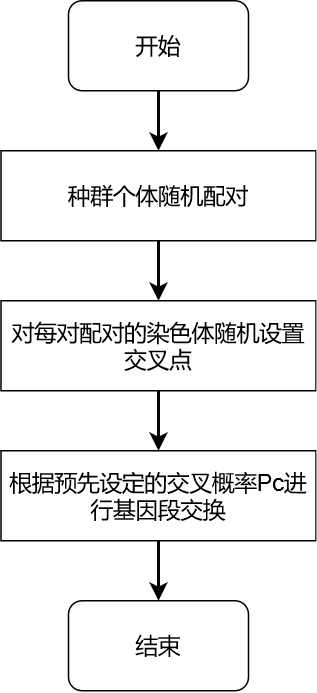
\includegraphics[width = 0.25\textwidth]{onepoint_cross.drawio.png}
  \caption{单点交叉流程图}
  \label{fig:onepoint_corss}
\end{figure}

其他类型的交叉操作还有双点和均匀交叉技术。双点交叉在匹配的染色体上随机确定两个位置,并将这两个位置之间的染色体段进行交换,以此来调整基因序列。
均匀交叉则对配对染色体上的每一个基因位都以相同的概率进行交叉,生成新的基因组合。
算术交叉通过对配对染色体执行线性组合的交叉,以产生变化的基因序列。
\begin{figure}[htbp]
  \centering
  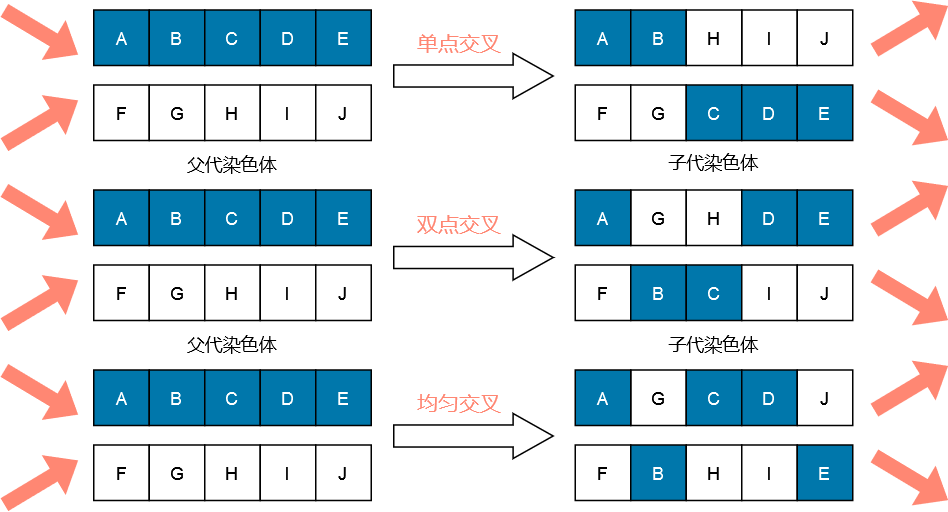
\includegraphics[width = 1.0\textwidth]{crossshow.drawio.png}
  \caption{交叉操作示意图}
  \label{fig:cross_show}
\end{figure}

\textbf{变异:}
为避免遗传算法过早收敛至局部最优,变异操作被引入以增强搜索的多样性。在应用中,常用的是单点变异,亦称位变异。
单点变异随机选取染色体上的一个基因位,并反转其值:若为二进制编码,则将0改为1,1改为0。
\begin{figure}[htbp]
  \centering
  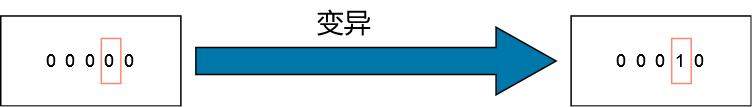
\includegraphics[width = 0.8\textwidth]{mutate.drawio.png}
  \caption{变异操作示意图}
  \label{fig:mutate}
\end{figure}

群体$P(t)$经过选择、交叉、变异运算后得到下一代群体$P(t+1)$。
若$t\leq T$,则 $t \leftarrow t + 1$,重新计算适应值;否则以进化过程中所得到的具有最大适应度的个体作为最好的解输出,终止运算。
图~\ref{fig:ga_procedure}~是整个遗传算法的流程图。
\begin{figure}[htbp]
  \centering
  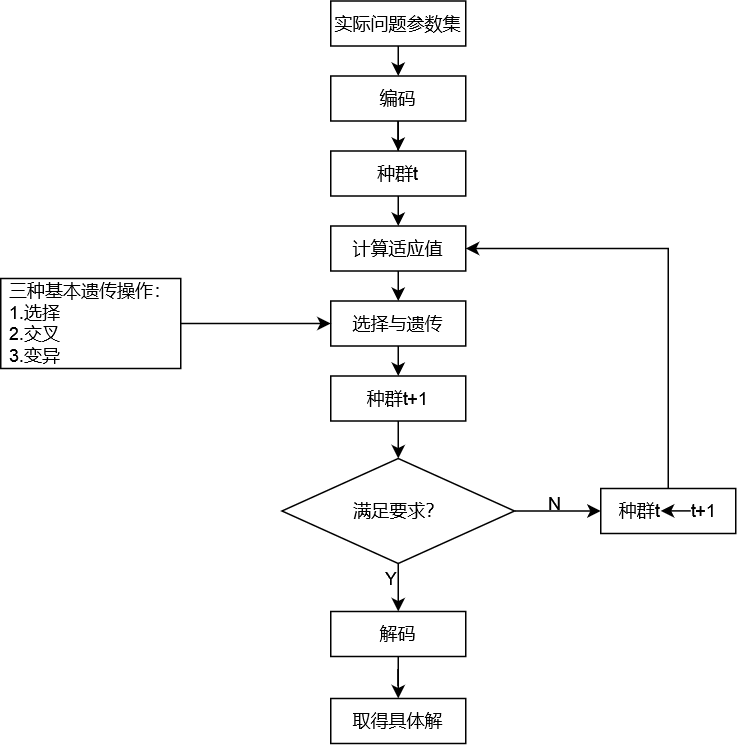
\includegraphics[width = 0.8\textwidth]{ga_procedure.drawio.png}
  \caption{遗传算法流程图}
  \label{fig:ga_procedure}
\end{figure}


\section{深度学习}
深度学习是机器学习的一个子集,它的算法受到人脑中的神经网络结构的启发,用于帮助机器识别模式和数据中的特征。
这种识别是通过一个多层次的抽象层完成的,每一层都会对信息进行加工和提炼,从而让机器能够理解复杂的数据,执行分类、识别等任务。

深度学习的核心构成是深度神经网络,这些网络除了包含输入层和输出层外,还嵌入了多个隐藏层,这种多层的叠加构造出了复杂且深远的网络结构。
图~\ref{fig:nerualnetwork}~展示了一个简单的神经网络结构。
在这一结构中,每一层都可以由众多节点或神经元组成,这些节点通过权重相互连接。
这些权重在训练过程中通过反向传播算法进行调整,以最小化预测和实际结果之间的差异。
这样的设计使得深度神经网络能够处理和学习大量复杂数据,从而在多种任务和应用中实现高度精确的预测和识别。

\begin{figure}[htbp]
  \centering
  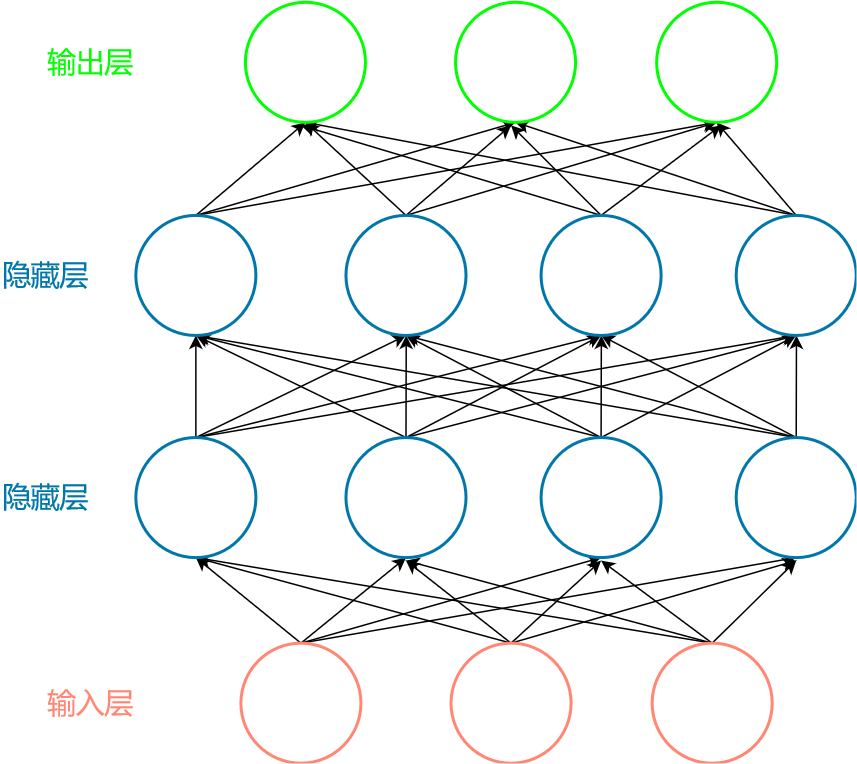
\includegraphics[width = 0.6\textwidth]{nerualnetwork.drawio.png}
  \caption{神经网络结构图}
  \label{fig:nerualnetwork}
\end{figure}

\subsection{卷积神经网络\cite{lecun1998gradient}}
卷积神经网络(Convolutional Neural Networks, CNNs)是一种专门用于处理具有类似网格结构数据的深度学习算法,最典型的应用是图像处理,其中数据可以被视为2D网格。
CNNs的设计灵感来源于生物的视觉皮层结构,特别是视觉皮层中那些负责处理光线、阴影、边缘等视觉元素的神经元的组织方式。

卷积神经网络的关键特性之一是其能够自动、有效地学习空间层次的特征。
这是通过网络中的卷积层来实现的,它们使用一组可学习的滤波器或卷积核扫描整个图像或信号。
这些滤波器能够捕捉到局部依赖性(例如边缘或纹理)和图像中的空间层次结构,使得CNN非常适合处理图像和视频数据。

CNN通常包含三种类型的层:卷积层、池化层和全连接层。
图~\ref{fig:cnnnetwork}~展示了一个简单的卷积神经网络结构。
卷积层负责提取图像中的特征;
池化层用于减少数据的空间大小,提高计算效率,同时保持重要的特征;
全连接层则用于将网络中的特征汇总,并进行最终的分类或回归分析。

\begin{figure}[htbp]
  \centering
  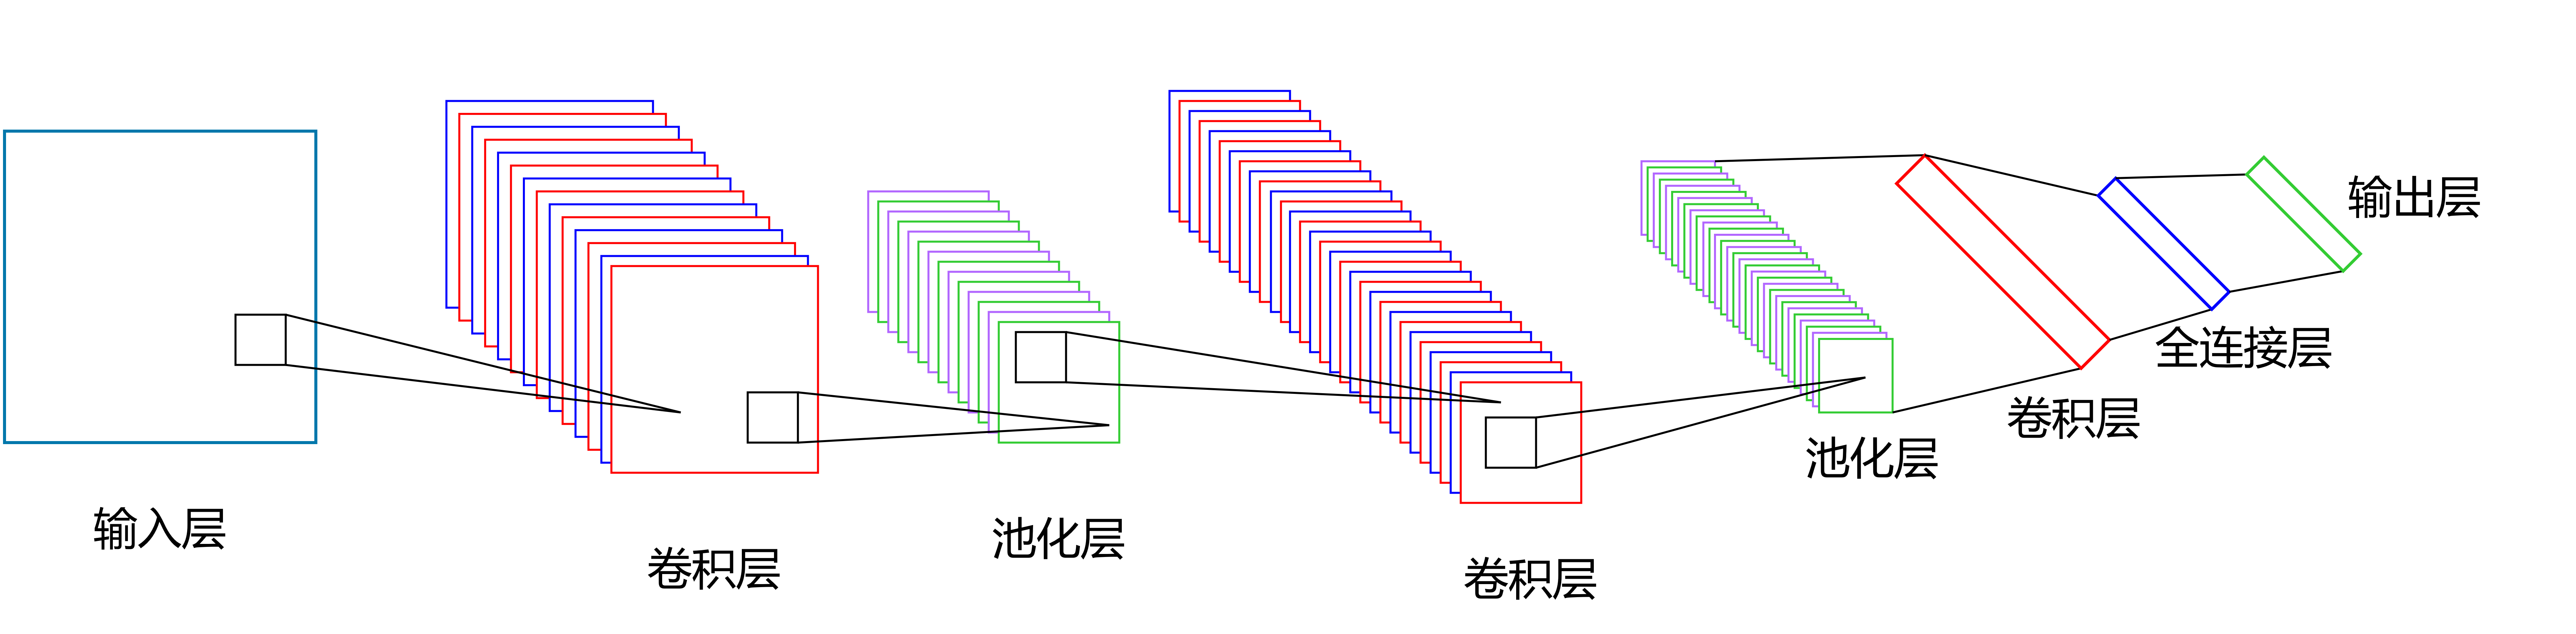
\includegraphics[width = 1.0\textwidth]{cnnstructure.drawio.png}
  \caption{卷积神经网络结构图}
  \label{fig:cnnnetwork}
\end{figure}

\subsubsection*{残差神经网络}
残差神经网络(Residual Neural Network,简称ResNet)是一种深度神经网络架构,它在2015年被提出,并且因其出色的性能获得了ImageNet大规模视觉识别挑战(ILSVRC)\footnote{http://image-net.org/challenges/LSVRC/2015/ 和 http://mscoco.org/dataset/\#detections-challenge2015.}的胜利\onlinecite{he2016deep}。
ResNet的核心思想是引入了“残差学习”的概念,以解决深度网络训练过程中的梯度消失或梯度爆炸问题,这使得我们能够成功地训练出比以往更深的网络模型,极大地提高了识别和分类任务的准确率。


如图~\ref{fig:traintesterror}~所示,在传统的深度神经网络中,随着层数的增加,网络变得越来越难以训练,这主要是因为梯度在反向传播时会逐渐消失或爆炸,导致网络权重难以更新。


\begin{figure}[h]
  \centering
  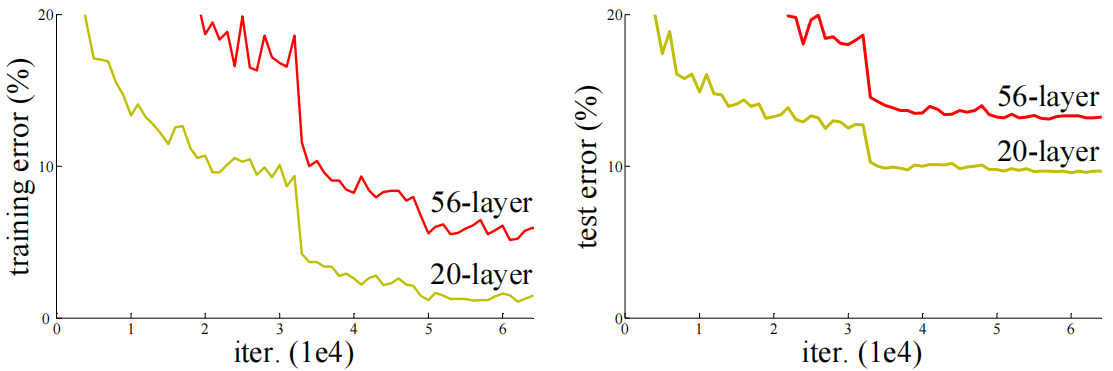
\includegraphics[width = 0.8\textwidth]{traintesterror.png}
  \caption{20层和56层的“普通”网络在CIFAR-10数据集上训练结果,左图是训练误差,右图是测试误差\cite{he2016deep}。}
  \label{fig:traintesterror}
\end{figure}

残差网络通过添加直接的跳跃连接(shortcut connections)来解决这个问题。
这些跳跃连接允许输入直接传递到后面几层中,从而在不同层之间创建了一条更短的路径。
跳跃连接(Shortcut Connections)是ResNet的标志性设计,它们使得输入可以跳过一层或多层直接传递到更深的层。
在实践中,这意味着深层网络能够学习到一个恒等映射,确保增加的层可以至少不会降低网络的性能。
这背后的原理是不再利用多层堆叠的块直接拟合一个期望的底层映射,而是明确让这个块拟合一个残差映射。
形式上,假设期望的底层映射为$H(x)$,而我们让堆叠的块拟合另一个映射,即残差映射:
\begin{equation}
  \label{eq:residual_mapping}
  F(x) := H(x) - x
\end{equation}
因此原始映射将被重新表述为$F(x) + x$。
这样做的好处是,优化残差映射比优化原始的、未引用的映射更容易。
图~\ref{fig:Resnetvsplai}~是18层、34层普通网络与残差网络在ImageNet数据集上训练误差与测试误差对比结果。
\begin{figure}[htbp]
  \centering
  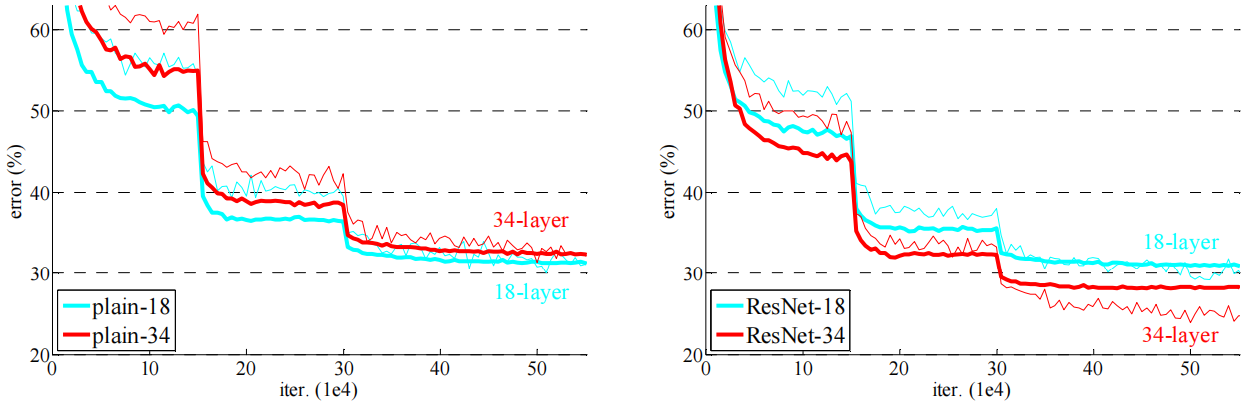
\includegraphics[width = 0.8\textwidth]{Resnetvsplain.png}
  \caption{18层、34层“普通”网络与残差网络在ImageNet数据集上训练误差与测试误差对比结果\cite{he2016deep}。}
  \label{fig:Resnetvsplai}
\end{figure}
可以看到残差网络相比层数相同的普通网络具有更好的训练效果以及更快的优化速度。



残差网络由多个残差块组成,每个块内部都有几层卷积层和一个跳跃连接。
图~\ref{fig:resnet_structure}~展示了一个由两层权重层堆叠的残差块。
\begin{figure}[htbp]
  \centering
  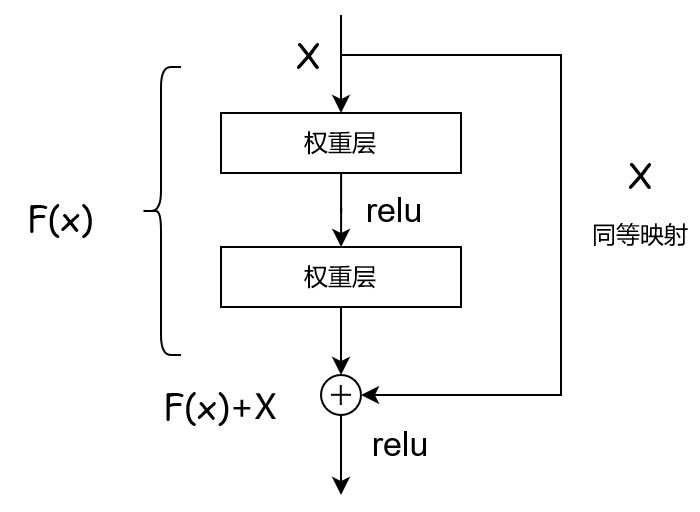
\includegraphics[width = 0.6\textwidth]{ResNet.drawio.png}
  \caption{两层堆叠的残差块结构图}
  \label{fig:resnet_structure}
\end{figure}
通过跳跃连接,ResNet解决了梯度消失和爆炸问题,使得训练深度模型成为可能。
ResNet允许我们构建更深的网络模型而不会降低性能,这在许多视觉识别任务中都实现了前所未有的准确率。
ResNet不仅在图像分类、检测和识别任务中表现出色,也被广泛应用于其他领域,如自然语言处理和音频分析。

\subsection{循环神经网络}
由于传统的神经网络主要由独立运作的输入层、隐藏层以及输出层构成,所以数据仅能在这些层间单向传递,这限制了其处理时间序列数据的能力。
对于那些数据内容随时间变化而紧密相关的场景,如视频、音频及文本等,传统神经网络难以有效捕捉其中的时序特征。
因此,为了克服这一限制并优化对时序数据的处理,研究者们提出了循环神经网络(Recurrent Neural Network,RNN)\onlinecite{lecun2015deep}。


RNN是一种专为处理序列数据而设计的神经网络架构。
与传统的前馈神经网络不同,RNN能够处理输入数据之间的时间动态性,使其特别适用于语言模型、语音识别、机器翻译等领域。
RNN的基本单元包括输入层、一个或多个循环隐藏层以及输出层。
RNN的基本单元结构如图~\ref{fig:RNNunit}~所示。
\begin{figure}[htbp] 
  \centering
  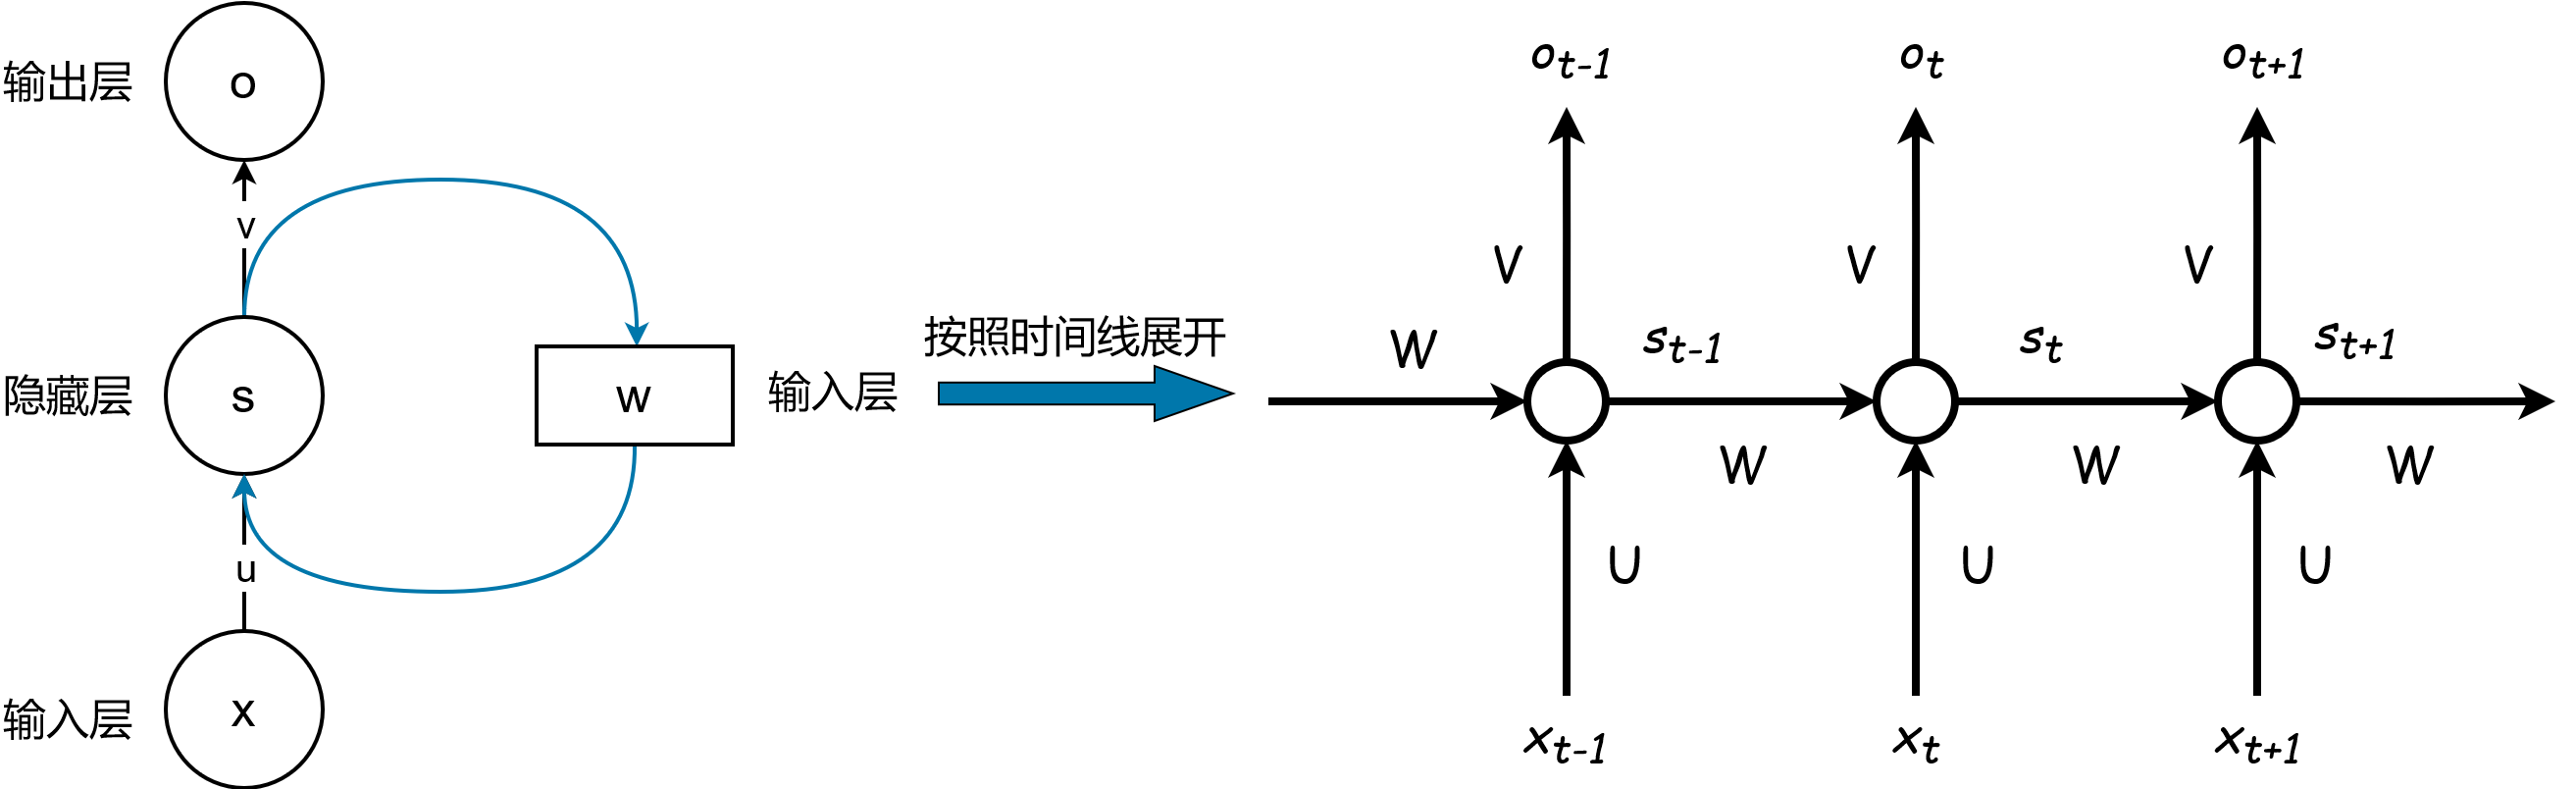
\includegraphics[width = 1.0\textwidth]{RNNunit.drawio.png}
  \caption{RNN基本单元结构图}
  \label{fig:RNNunit}
\end{figure}


由于RNN的网络结构设计允许在处理序列数据时,将前一时间步的信息传递到当前时间步,这使得RNN具备短期记忆能力。
这种能力主要通过网络中的隐藏层状态实现,其中每个时间步的隐藏状态都依赖于前一个时间步的隐藏状态和当前时间步的输入。
具体来说,RNN的每个时间步都会接收两个输入:当前时间步的数据输入和前一时间步的隐藏层状态。
例如,在 t 时刻,输入层将$x_t$输入到隐藏层$s_t$的同时,隐藏层的上一个输出$s_{t-1}$也作为输入,输入到隐藏层$s_t$中。
由此,t 时刻的输出和隐藏层的值计算方式如公式~\ref{eq:RNN_ot}、\ref{eq:RNN_st}~所示:
\begin{gather}
  O_t = g(V \cdot S_t) \label{eq:RNN_ot} \\
  S_t = f(U \cdot X_t + W \cdot S_{t-1}) \label{eq:RNN_st}
\end{gather}
\begin{flushleft}
  \renewcommand\arraystretch{1.25}
  \begin{tabularx}{\textwidth}{@{}>{\normalsize\rm}l@{\quad}>{\normalsize\rm}l@{——}>{\normalsize\rm}X@{}}
  式中
  &  $g$ &输出层神经元激活函数;\\
  &  $f$ &隐藏层神经元激活函数;\\
  &  $V$   &隐藏层到输出层权重参数;\\
  &  $U$ & 输入层到隐藏层权重参数;\\
  &  $W$ & t-1时刻隐藏层输出到t时刻隐藏层输出权重参数;\\
  &  $x_t$ &t时刻输入;\\
  &  $s_t$ & t时刻隐藏层输出;\\
  \end{tabularx}\vspace{.5ex}%TODO : 注释内容自动转页接排
\end{flushleft}

这个隐藏层状态包含了之前时间步的信息,相当于网络的“记忆”。
然后,RNN通过当前的输入和这份“记忆”来更新其隐藏状态,以及生成当前时间步的输出。
通过这种机制,RNN能够在处理每个时间步的数据时,考虑到序列之前的信息,实现对信息的短期记忆。

\subsubsection*{门控循环单元}
虽然RNN理论上能够捕捉序列中的长距离依赖关系,但在实践中,由于梯度消失或梯度爆炸的问题,其实际的记忆能力往往被限制在较短的序列上。
所以后来的研究者门提出了如长短期记忆网络(LSTM)\cite{memory2010long}和门控循环单元(GRU)\cite{cho2014learning}等更高级的循环网络结构,它们通过特殊的设计来显著提高网络对长期依赖关系的捕捉能力。
LSTM 通过门控机制使循环神经网络不仅能记忆过去的信息,同时还能选择性地忘记一些不重要的信息而对长期语境等关系进行建模,而 GRU 基于这样的想法在保留长期序列信息下减少梯度消失问题。
相比LSTM,使用GRU能够达到相当的效果,并且相比之下更容易进行训练,能够很大程度上提高训练效率,因此很多时候会更倾向于使用GRU。

图~\ref{fig:GRUunit}~是GRU基本单元的组成结构图。
\begin{figure}[htbp] 
  \centering
  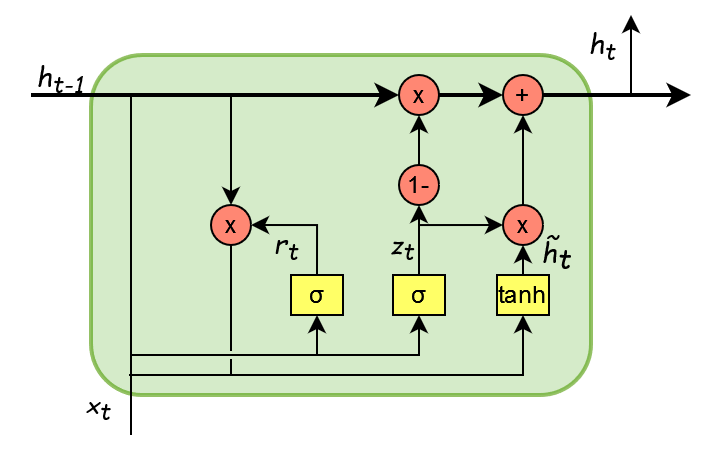
\includegraphics[width = 0.8\textwidth]{gru.drawio.png}
  \caption{GRU基本单元结构图}
  \label{fig:GRUunit}
\end{figure}
\begin{flushleft}
  \renewcommand\arraystretch{1.25}
  \begin{tabularx}{\textwidth}{@{}>{\normalsize\rm}l@{\quad}>{\normalsize\rm}l@{——}>{\normalsize\rm}X@{}}
  图~\ref{fig:GRUunit}~中
  &  $\times$ &Hadamard Product,矩阵相乘运算;\\
  &  $+$ &矩阵加法运算;\\
  &  $σ$ &Sigmoid 激活函数,输出范围为0 -- 1;\\
  &  $\tanh$ & $\tanh$激活函数,输出范围为-1 -- 1;\\
  \end{tabularx}\vspace{.5ex}%TODO : 注释内容自动转页接排
\end{flushleft}

GRU由\textbf{重置门(reset gate)}和\textbf{更新门(update gate)}两种类型的门控机制构成。
这些门控制着信息的流动,决定了哪些信息应当被保留,哪些信息应当被忽略或删除,从而有效地捕捉到长期依赖性。

其中,重置门决定了多少过去的信息需要被忘记。
它允许模型抛弃与新信息无关的旧状态信息,使模型能够更灵活地处理每个时间点的数据。
GRU得到门控信号$r_t$之后,首先使用重置门控来得到“重置”之后的数据$h'_{t-1} = r_t \cdot h_{t-1}$,再将$h'_{t-1}$与输入$x_t$进行拼接,再通过一个$\tanh$激活函数来将数据放缩到-1 -- 1的范围内。
这一过程如公式~\ref{eq:gru_rt}、\ref{eq:gru_ht}~所述。
\begin{gather}
  r_t = σ(W_r \odot [h_{t-1},x_t]) \label{eq:gru_rt} \\
  \tilde{h_t} = \tanh(W \odot [r_t \cdot h_{t-1} , x_t]) \label{eq:gru_ht}
\end{gather}
这里的$h'_{t-1}$主要是包含了当前输入的$x_t$数据。
有针对性地对$h'_{t-1}$添加到当前的隐藏状态,相当于“记忆了当前时刻的状态”。
类似于LSTM的选择记忆阶段。


更新门帮助模型决定过去的信息有多少需要保留到未来。
它在决定状态信息是否更新时起着关键作用,类似于LSTM中的遗忘门和输入门的组合。
“更新记忆”阶段是GRU最关键的一个阶段。
在这个阶段,GRU同时进行了遗忘与记忆两个步骤。
我们使用了先前得到的更新门控$z$得到更新表达式: 
\begin{equation}
  \label{dq:gru_ht}
  h_t = (1-z) \odot h_{t-1} + z \odot h'_{t-1}
\end{equation}
门控信号$z$的范围为0 -- 1。门控信号越接近1,代表“记忆”下来的数据越多;而越接近0则代表“遗忘”的越多。
可以看到,这里的遗忘$z$和选择$(1-z)$是联动的。
也就是说,对于传递进来的维度信息,我们会进行选择性遗忘,则遗忘了多少权重($z$),GRU就会使用包含当前输入的$h'_{t-1}$中所对应的权重进行弥补。
以保持一种“恒定”状态。

\subsubsection*{双向门控循环单元}

\begin{figure}[htbp]
  \centering
  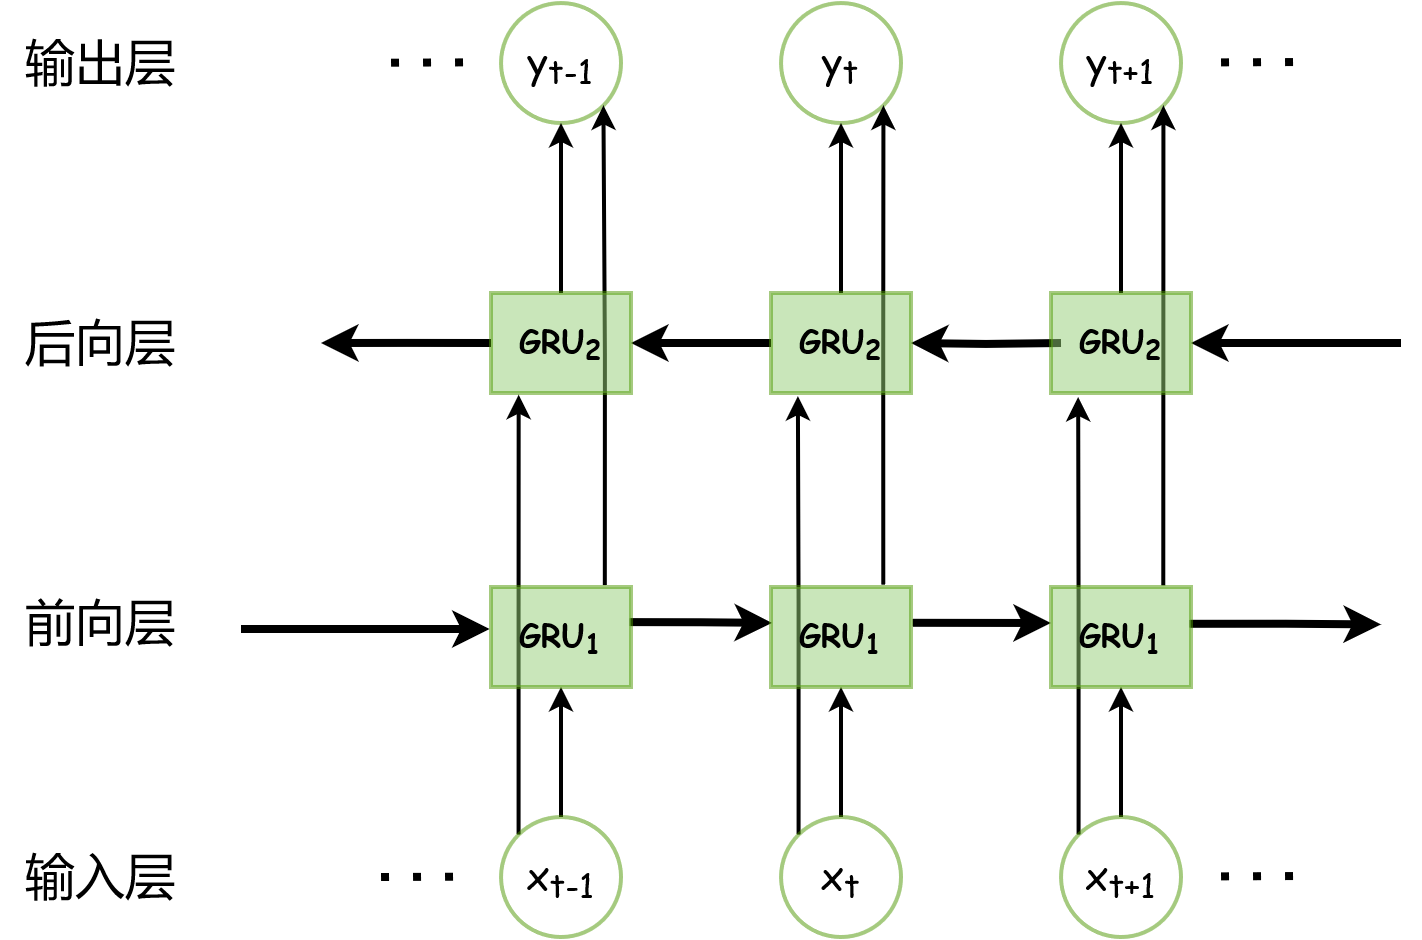
\includegraphics[width = 0.8\textwidth]{BiGRU.drawio.png}
  \caption{BiGRU结构图}
  \label{fig:BiGRU}
\end{figure}

双向门控循环单元(Bidirectional Gated Recurrent Unit, BiGRU)是一种特殊类型的循环神经网络(RNN)结构,它结合了GRU(门控循环单元)的优势和双向RNN的特点,以更有效地处理序列数据。
BiGRU通过同时处理过去和未来的信息,能够在序列处理任务中,如自然语言处理(NLP)和语音识别,提供更丰富的上下文信息。


BiGRU除了具备GRU的门控机制之外另一个核心特点是核心特点是双向处理。
图~\ref{fig:GRUunit}~展示的是一个沿着时间展开的双向循环神经网络。
BiGRU包含两个GRU层,一个沿正时间方向处理数据(正向GRU),捕捉从过去到现在的依赖;
另一个沿反时间方向处理数据(反向GRU),捕捉从未来到现在的依赖。
这两个层的输出通常会在每个时间步被合并,以提供给定时间点前后的完整上下文信息。
另外,从GRU继承的更新门和重置门可以使模型在每个方向上更有效地学习长期和短期依赖性。

对于一个输入序列 $X = x_1 x_2 \dots x_T$,BiGRU模型的前向计算可以表示为:
\begin{gather}
  \overleftarrow{h_t} = GRU_1(x_t,\overleftarrow{h_{t-1}}) \label{eq:bigru_htleft} \\
  \overrightarrow{h_t} = GRU_1(x_t,\overrightarrow{h_{t-1}}) \label{eq:bigru_htright} \\
  y_t = \overleftarrow{h_t} \oplus \overrightarrow{h_t} \label{eq:bigru_out}
\end{gather}
\begin{flushleft}
  \renewcommand\arraystretch{1.25}
  \begin{tabularx}{\textwidth}{@{}>{\normalsize\rm}l@{\quad}>{\normalsize\rm}l@{——}>{\normalsize\rm}X@{}}
  其中
  &  $y_t$ &模型输出;\\
  &  $\overrightarrow{h_t}$ &前向输出;\\
  &  $\overleftarrow{h_t} $ &后向输出;\\
  &  $\oplus$ & element-wise sum按位加。\\
  \end{tabularx}\vspace{.5ex}%TODO : 注释内容自动转页接排
\end{flushleft}

